\section{Real World application}

A general s-plex application that is probably used is the identification of group or friend networks
where one can make assumptions about group or friend networks. This is application is not directly
derived from our programming assignment, but it is somewhat related since one still has to identify k-plexes in a
undirected graph which with the amount of people using social media these days is not trivial.
An application that is closer to the given s-plex programming assignment would be telecommunication networks.
Where the distance between the antennas, towers or compute node could be correlated to the weight matrix and the s-plex
relaxation of the clique's could be used to make crucial system more reduntant (low s-plexes) and other less crucial systems
less reduntant (higher s-plexes).

\section{Deterministic Construction Heuristic}

Our first idea for a construction of solutions is the following: An empty graph (without edges) is always 
a 1-plex, since a single node without edges is a 1-plex. Removing all the edges gives a valid solution, 
however a very bad one. Our first idea for an algorithm that finds a good solution was to start with an 
empty graph and go through all the edges in $A_0$, check if adding them to $A$ is legal and if so, do that. 
This algorithm improves the empty graph, however it can only find $s$-plexes of up to $|S|=s+1$. The reason 
is that it will connect the first node $v_1$ with $\min(s,\deg_{A_0} (v_1))$ many other nodes, then the 
cluster of $v_1$ is an $s$-plex with size at most $s+1$ and no more nodes can be added. Then, all the other 
nodes in the cluster might get connected among each other, but the $s$-plex will not get any bigger. 
Practically speaking, with this construction we got approximately $n/(s+1)$ many clusters of size $s+1$ 
which were mostly fully connected, so this construction results in small clusters.\\

\textcolor{red}{
deterministic construction heuristic where we explain how the construction heuristic is done.
Maybe only do on the problem with 9 vertices and plot some results.}

\pagebreak

\section{Randomized Construction Heuristic}

For our random construction we randomly parse the entries of $A_0$ but do the same as above otherwise.

\subsection{Local improvement move operators}
After this point we found it difficult to think of the next move, because simply adding one edge in this state 
will always yield an illegal solution. In trying to understand the problem better, we wrote the adjacency 
matrices $A_0$ in files and looked at their structure. What we found was that there is a structure in most of the 
graphs, more precisely there are 3 types of graphs (see also figure \ref{fig:types}):

\begin{enumerate}
    \item locally strongly connected: 26/60 (Here, nodes that are close in numbering are also strongly connected 
    in the graph)
    \item seemingly randomly connected: 23/60
    \item tentacle-like connected: 7/60 (Here, the Graphs have a semi-large, strongly 
    connected cluster with "tentacles" reaching out. Tentacle-shaped clusters are bad for $s$-plexes, 
    so we will have to seperate these "lines" into small "spheres".)
\end{enumerate}

\begin{figure}[h]
\centering
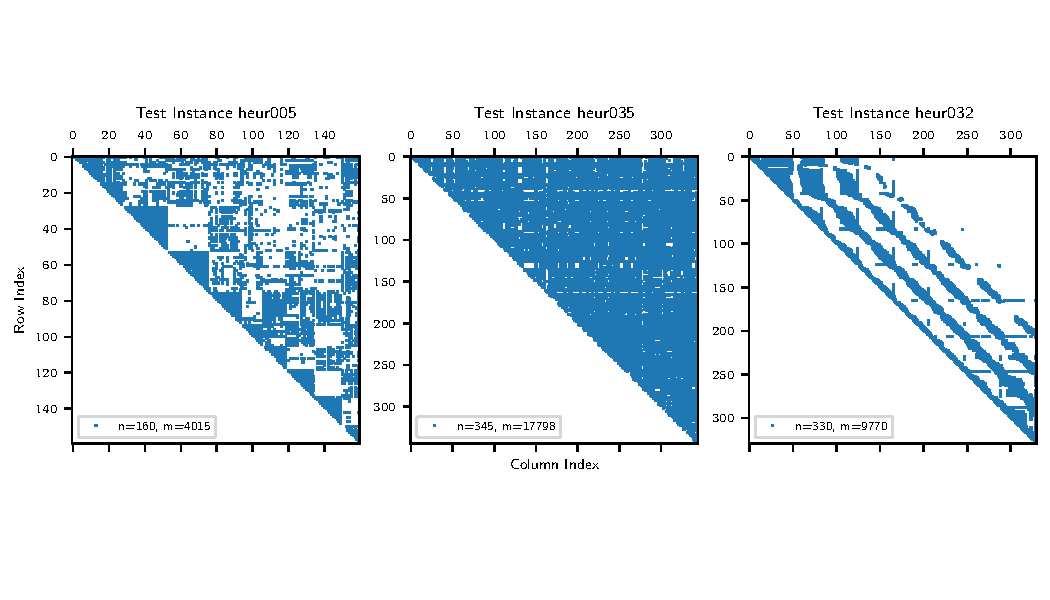
\includegraphics[width=\linewidth, trim= {0 1.8cm 0 1.8cm}, clip]{figures/spy_adjacency.pdf}
\caption{\label{fig:types}Instances of the different graph types. Left is a locally strongly 
connected graph, this is part of instance 005. In the middle is a seemingly randomly connected graph, 
which is part of instance 035. On the right is a tentacle-like connected graph, which is part of instance 032.}
\end{figure}

We will use this special structure of some instances to derive parts of our algorithms. Some might consider 
this cheating, but we think, that finding patterns in the instances is an important part of solving problems 
in real world applications so we find it to be okay. We will see later, that for the locally strongly connected 
instances we can find reasonably good solutions with very little computational effort. We will also see that 
the algorithms that were derived with the locally connected graphs in mind also work well on the other graphs.\\

\pagebreak

\subsubsection{Fuse Operation}
The case of locally strongly connected graphs made it easier to think about the problem. The idea for our next move came 
from looking at the following situation. Let's say we are looking for 2-plexes and a certain section of our adjacency 
matrix is a clique, so $A_0$ in that part looks like\\

\begin{figure}[h]
    \begin{subfigure}{0.5\textwidth}
        \centering
        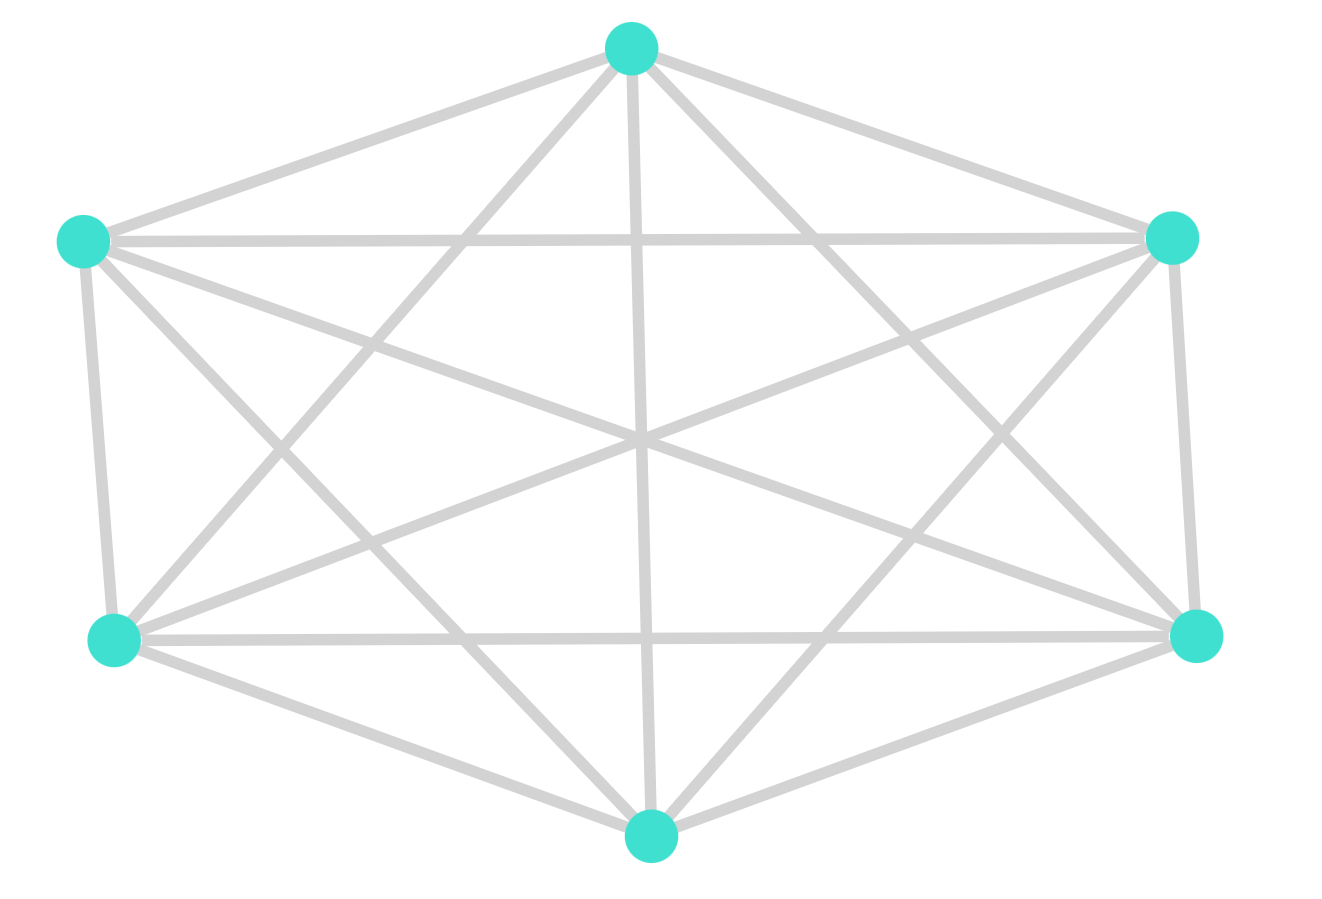
\includegraphics[width=0.8\linewidth]{figures/A0.PNG}
        \caption{Graph with A0 Adjacency Matrix}
        \label{fig:sub1}
    \end{subfigure}%
    \begin{subfigure}{0.5\textwidth}
        \centering
        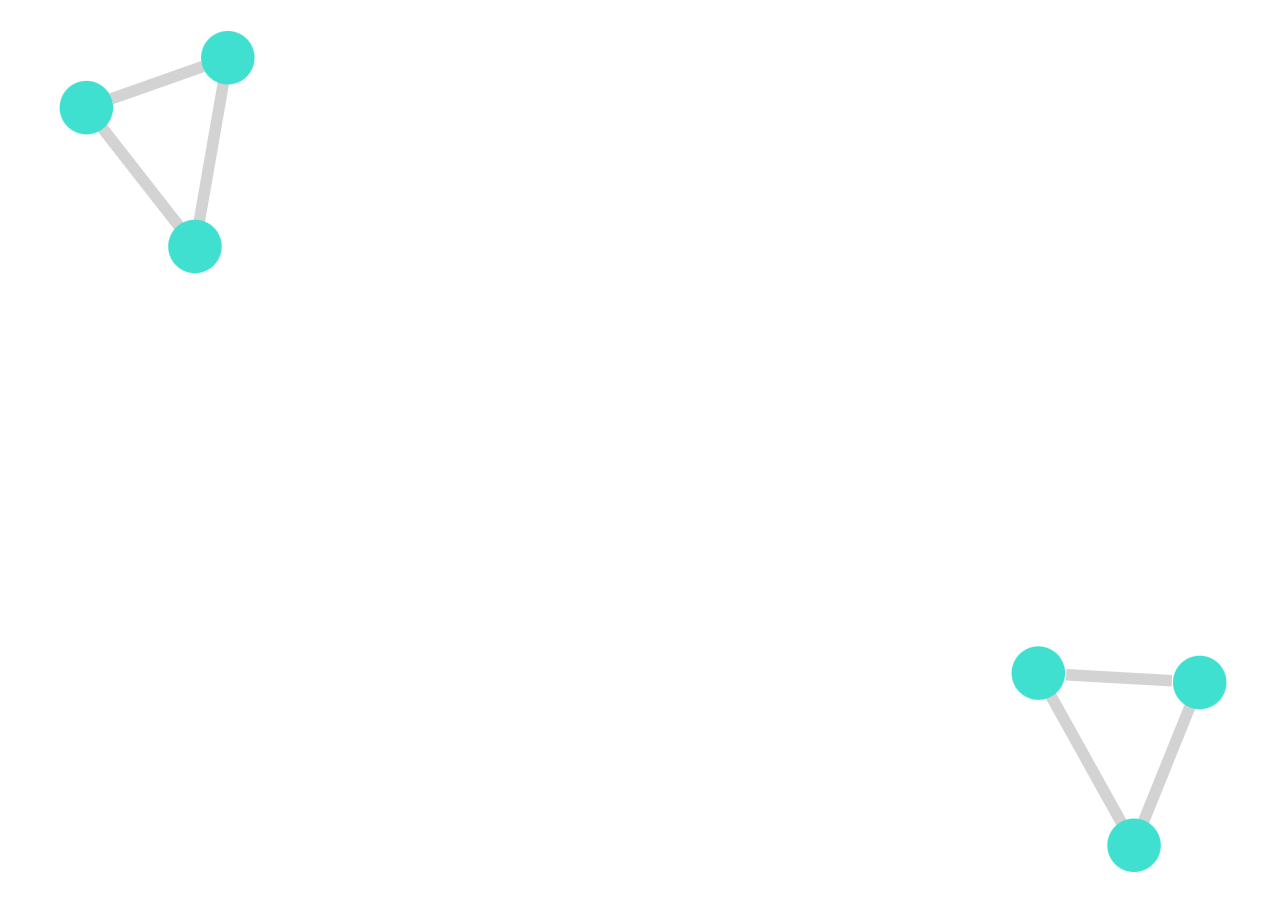
\includegraphics[width=0.8\linewidth]{figures/A.PNG}
        \caption{Solution A based on A0}
        \label{fig:sub2}
    \end{subfigure}
    \caption{Caption for the entire figure.}
    \label{fig:full}
\end{figure}


To get from our constructed $A$ to $A_0$ in this section we need to set to 1 all the entries between the 2 cliques. 
In terms of the graph, we fully connect the two found cliques. Exactly this is our idea for the first move, which is 
then also applicable for the randomly distributed graphs.\\
So our first move after construction is fully connecting existing clusters, this always yields a legal $s$-plex. We 
call this operation a \textbf{fuse} the corrsponding functions are called \texttt{fuse\_first!} for first improvement 
and \texttt{fuse\_best!} for best improvement. We implemented this operation in a way, that it can fuse any 2 clusters, 
not only neighbouring ones.\\
Especially for the locally connected instances we found this to work very well and after repeatedly fusing clusters, 
our found adjecency matrices $A$ showed very similar structures to the original ones $A_0$.\\
After fusing two clusters one could also try to remove edges that are not there in $A_0$ until no more edges can be 
removed legally. We describe our strategy for this in section \ref{sec:cliquify}. To do this after every move, set the 
global variable \texttt{SPARSEN} to true in \texttt{move\_ops.jl} (as we said above: the code is very raw). We found 
that setting this to true improves the results slightly but greatly decreases performance (but we should mention here 
that we also implemented this in a very inefficient way). We decided that for good results it is sufficient to let 
the fuse method fully connect it's clusters and only at the end of the algorithm take out the unnecessary 
edges (see section \ref{sec:cliquify}).

\pagebreak

\null

\subsubsection{Swap Operation}
Looking at our results we found that in some cases, single nodes did not land in the cluster they were supposed 
to be in, for example in the case of instance 051 we found the solution given in figure \ref{fig:051_swap}.\\
\null
\begin{figure}[h]
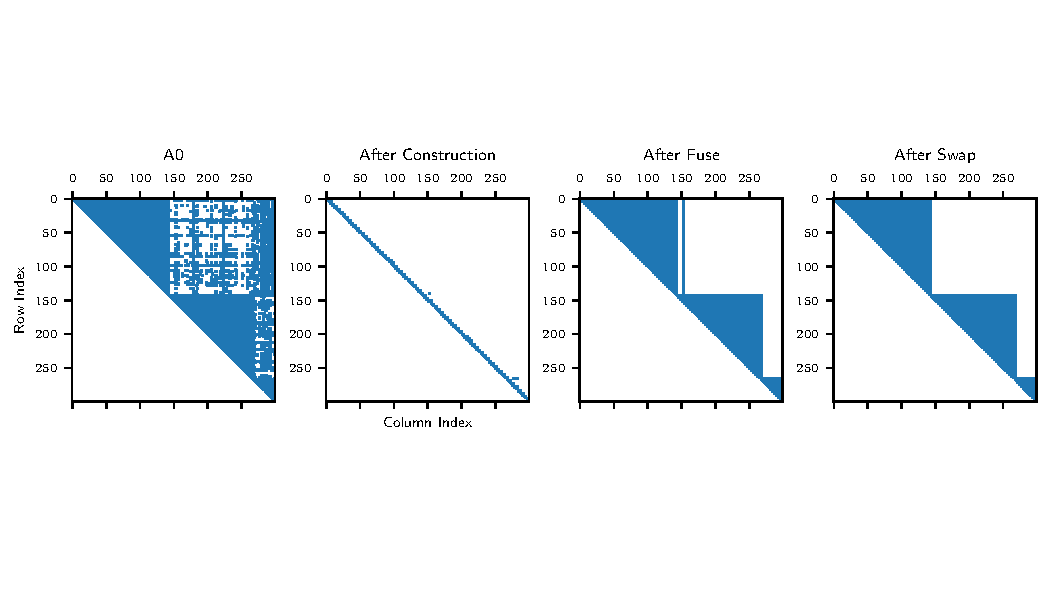
\includegraphics[width=\linewidth, trim= {0 3cm 0 0.9cm}]{figures/spy_adjacency2.pdf}
\caption{\label{fig:051_swap} Instance 051 after fusing until no progress is made. One can see that node 154 seems misplaced. Indeed, when node 154 is swaped to the other cluster the cost is reduced by roughly 500.}
\end{figure}

We see that node 154 looks a little misplaced and should be in the first cluster note the second one. 
When we manually put it into the first one we found that this indeed reduced the cost from 8645 to 8153 
which is a very significant improvement. So for our second move we think that it should be beneficial to 
try to swap nodes between clusters.\\

\subsubsection{Operation for taking our redundant edges}
\label{sec:cliquify}
All the discribed algorithms so far rather find cliques than s-plexes. In the fuse method, the clusters get 
fully connected, so any deviation from a clique must be in the original small clusters from the construction 
heuristic. Our algorithm finds clusters that are also clustered in $A_0$ but up till now it does not deal well 
with the edges in $A_0$ that are missing within a cluster. Generally, the most profitable edges in a cluster 
to remove will not always be in the small cluster from the construction heuristic. To find these most profitable 
edges to remove we implemented the \textbf{cliquify then sparsen} method. This method first fully connects the 
clusters within $A$ and then removes as many edges as possible, starting from the most profitable edges. This 
does not really fit into the framwork of metaheuristics, that we saw in the lecture, since it is more of a 
"cleanup" at the end of the search algorithm. One could also do one \textbf{cliquify then sparsen} after each 
however, this is again connected to more computational effort.\\

\subsubsection{Shaking operation}  
For the shaking operation for GVNS we thought that randomly disconnecting $n$ nodes totally might be a good idea. 
We implemented this an we will discuss it in the results section.\\

\subsubsection{Final thoughts}
In the case of the locally strongly connected graphs, our deterministic construction with a first improvement 
fuse strategy already works very well while being very efficient. The deterministic construction which goes 
through the nodes by their numbering and thereby clusters them mostly right, since nodes that are close in numbering 
are also "close" in the graph. The first improvement fuse operation will then first fuse the clusters which 
are closest in numbering, which also fits the structure of these graphs.\\
In the case of seemingly randomly connected graphs, the numbering is not correlated to how close nodes are in the 
graph, so here a random construction with GRASP, that rather randomly groups nodes in the beginning should perform 
better. For the same reason, a best improvement strategy for the fuse-operation should be better, however, this is 
very costly in terms of computation.\\
From our discussion above, we come to the conclusion, that first progressively fusing clusters until there is node 
more profit to make from fusing and then swapping the misplaced nodes until there is no more profit to make is a 
reasonable strategy here. Since there was no metaheuristic discussed in the lecture that exactly fits this procedure 
we will call it \textbf{sequential local search} (SNS) because we sequentially apply move operators. It is somewhat 
of a mix of local search and VND. We will also compare this metaheuristic to the other ones. Our expectation is that 
the results will be worse than for e.g. VND but that the computational performance will be significantly better.\\